\newpage
\hypertarget{enums vis}{}
\subsection{Creating Enums in Enterprise Architect}
\visHeader

\begin{itemize}

\item[$\blacktriangleright$]
Let's start with the double-linked list demonstration specification, which is
readily provided with eMoflon:
Create a new meta-model project (``File/New/Other\dots", then ``eMoflon/New
Metamodel Wizard''), call your project ``Demo'', and tick ``Add Demo
Specification''.

\item[$\blacktriangleright$]
Open the EAP file ``Demo.eap'' and navigate to the diagram
``org.\-moflon.\-demo.\-doublelinkedlist''.

\item[$\blacktriangleright$]
Now, add a new ``EEnum'' type called color.
This can be done via the Toolbox (``Diagram/Toolbox'') or by pressing space
while the cursor is inside the digram area.
Your diagram should resemble Figure~\ref{enums:vis:createEEnum}.

\begin{figure}[htbp]
    \begin{center} 
        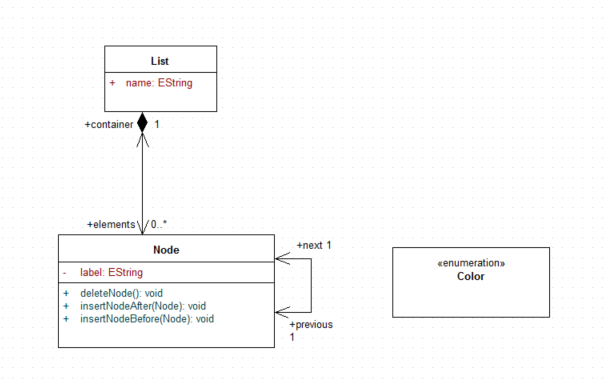
\includegraphics[width=.8\textwidth]{visCreateEEnum}
        \caption{Creating a new EEnum}  
        \label{enums:vis:createEEnum}
    \end{center}
\end{figure}

\item[$\blacktriangleright$]
We now create the three colors that our list nodes may have.
An enum constant is a special attribute.
Therefore, open the attriutes view of \texttt{Color} (``Right-click/Features \&
Properties/Attributes\dots'') and add three attributes as shown in
Figure~\ref{enums:vis:enumAttributes}.
Make sure that the type of the attributes is \texttt{Color} and that each
attribute has an ``initial value''.

\begin{figure}[htbp]
    \begin{center} 
        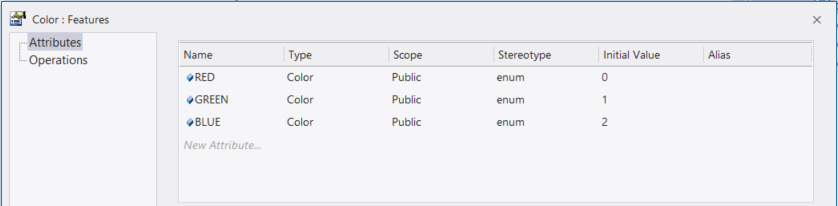
\includegraphics[width=.8\textwidth]{visEnumAttributes}
        \caption{Creating the three color attributes \texttt{RED},
        \texttt{GREEN}, and \texttt{BLUE}}
        \label{enums:vis:enumAttributes}
    \end{center}
\end{figure}

\item[$\blacktriangleright$]
Finally, create a \texttt{color} attribute of type \texttt{Color} in EClass
\texttt{Node} (Figure~\ref{enums:vis:colorAttribute}).


\begin{figure}[htbp]
    \begin{center} 
        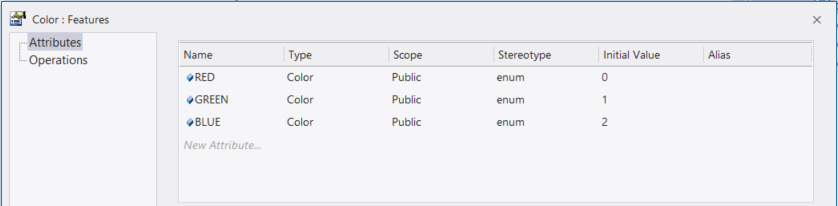
\includegraphics[width=.8\textwidth]{visEnumAttributes}
        \caption{\texttt{color} attribute of EClass \texttt{Node}}
        \label{enums:vis:colorAttribute}
    \end{center}
\end{figure}

\item[$\blacktriangleright$]
Validate and export and build your metamodel.

\item[$\blacktriangleright$]
A minimal test for the new feature could be implemented in the class
\texttt{NodeTest} as follows:
\begin{lstlisting}[language=Java,caption={Test for coloring nodes}]
@Test
public void testAddColor() throws Exception {
	Node node = 
	    DoublelinkedlistFactory.eINSTANCE.createNode();
	node.setColor(Color.RED);
}
\end{lstlisting}

\end{itemize}